\subsection*{Explicación}
Para este ejercicio seguí la misma lógica del ejercicio 1 pero obviando el DEMUX 1:8.

\subsection*{Código}
\faGithub \space
\href{https://github.com/warleon/Arch-lab1/tree/master/pregunta2}{https://github.com/warleon/Arch-lab1/tree/master/pregunta2}\\
make DEMUX\_1\_16
%\subsection*{Tabla de verdad}

%\subsection*{Mapa de Karnaugh}

%\subsection*{Ecuaciones booleanas}

\subsection*{Resultados}
\begin{figure}[h]
    \centering
    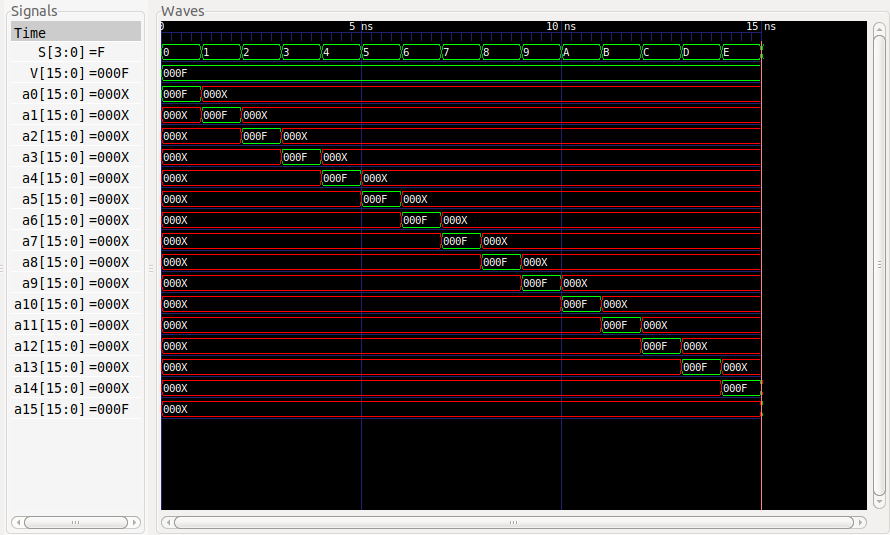
\includegraphics[scale=0.5]{fotos/resultados/arki-DEMUX_1_16.png}
    \caption{waves demux 1:16}
\end{figure}